
\documentclass{beamer}
\usepackage{graphicx}


%Global Background must be put in preamble


\usetheme{Madrid}

\title{COP 290}

\subtitle{Designing Documentation}

\author{Ayushya Raj \and Nitin Rathor \and Ankush Phulia}

\institute[IIT Delhi] 
{
  Department of Computer Science\\
  IIT Delhi}

\subject{COP 290}



\begin{document}

{\usebackgroundtemplate%
{
\includegraphics[width=\paperwidth,height=\paperheight]{back.png}}
\begin{frame}
  \titlepage
\end{frame}
}
{\usebackgroundtemplate%
{
\includegraphics[width=\paperwidth,height=\paperheight]{back.png}}
\begin{frame}{Application Description}{}
  \begin{itemize}
  \item {
   A basic registration application consisting of two screens- a welcome and a main registry page where all the details have to be filled.
  }
  \item {
    Divided into two activities and three classes, along with various design layouts and resources for various parts of the user interface
  }
  \item {
    Checks for an incomplete form, that is, empty fields and invalid entries, have been introduced and visually any problems in the form filling through a variety of ways
  }
  \item{
  Volley network library used (as encouraged) to send and receive data from the server, if all the details are properly provided
  }
  \end{itemize}
\end{frame}
}
{\usebackgroundtemplate%
{
\includegraphics[width=\paperwidth,height=\paperheight]{back.png}}

\begin{frame}{Application Features}
  \begin{itemize}
  \item {
    Required fields are indicated by an asterisk which does not go away till they have been filled. Should they be ignored, the user is reminded via a message in the text field itself when they try to proceed
  }
  \item {   
    For entry numbers, if invalid entries are provided, an alert box informing the user of the same is displayed, with focus going directly to the field in question and the invalid entry being cleared
  }
  \item {
    Selecting an already filled field selects all the text, allowing easy deletion
  }
  \item {
    Of course, the form is scrollable and each screen has a corresponding landscape layout
  }
  \item {
    On registry, the app displays a toast with the message it receives from the server. In case, registry is successful or the user is already registered, it goes back to its welcome screen, else it stays there.
  }
  \end{itemize}
\end{frame}
}
{\usebackgroundtemplate%
{
\includegraphics[width=\paperwidth,height=\paperheight]{back.png}}

\begin{frame}{High Level Functions Used }
\begin{block}{IsValid (String)}
To check if entry number given is valid.
\end{block}
\begin{block}{Text-Watcher Methods}
Added to various text fields to bring them into focus or hide the asterisk, indicating they are filled.
\end{block}
\begin{block}{On Click Methods}
For buttons which involve navigation, checking and sending requests to servers.
\end{block}
\begin{block}{Various Methods for Request Queue}
A separate class used to implement a global request queue in order to avoid creating a new one on every button click.
\end{block}


\end{frame}
}

\begin{frame}{How to use the app ? }
    \begin{enumerate}
        \item  
        \item 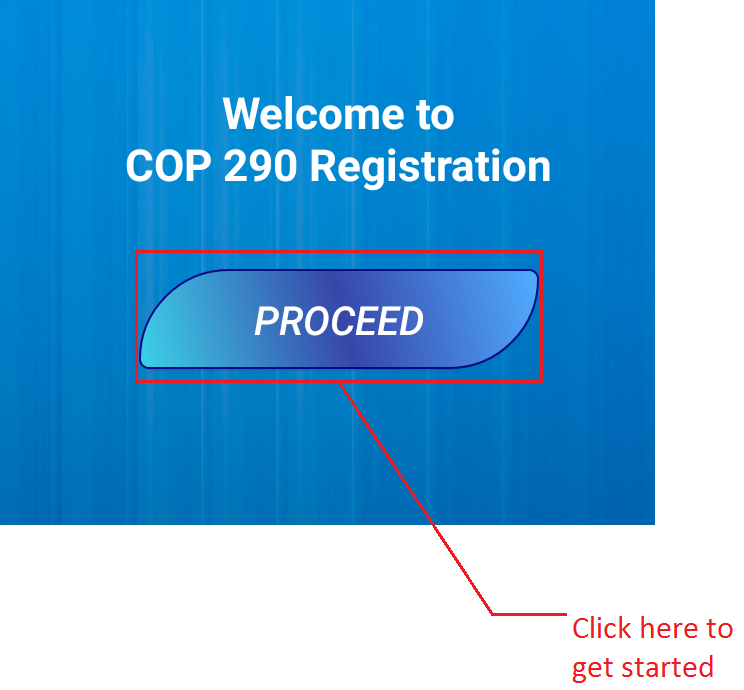
\includegraphics[scale = 0.153]{img1.png}        
        \item 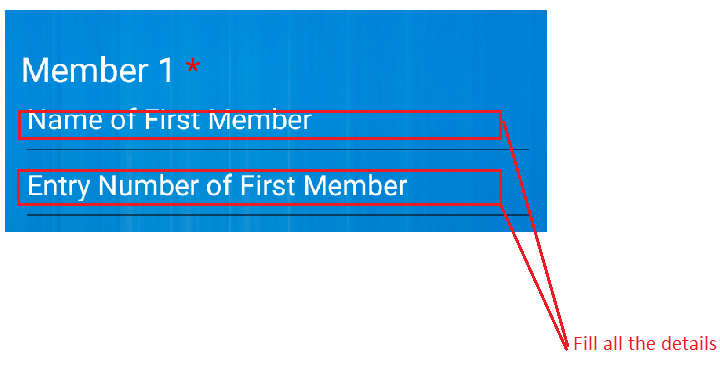
\includegraphics[scale = 0.25]{img2.png}
        \item 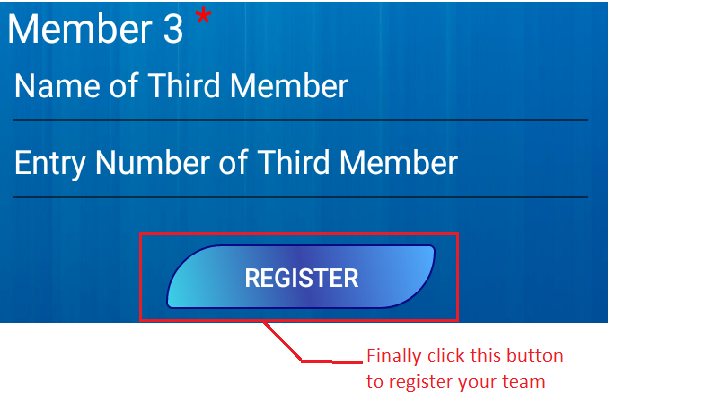
\includegraphics[scale = 0.225]{img3.png}
    \end{enumerate}
    
    
    
    
\end{frame}

{\usebackgroundtemplate%
{
\includegraphics[width=\paperwidth,height=\paperheight]{back.png}}

\begin{frame}{References}
    
    \begin{itemize}
        \item {Basic Reference:\\developer.android.com/training/}
        \item {Volley References :\\ developer.android.com, androidhive.info}
        \item {Icon Images and Backgrounds:\\ tradefair.omaheke.com, tophdimg.com }
        \item {Miscellaneous methods and troubleshooting :\\ Android Documentation, Stack Overflow}
    \end{itemize}
    
\end{frame}
}

\end{document}


